\begin{frame}{Języki dedykowane pod Code Golf}
    % \begin{itemize}
    %     \myitem GolfScript
    %     \myitem MetaGolfScript
    % \end{itemize}

    {\large GolfScript}

    \begin{itemize}
        \myitem Darren Smith, 2007
        \myitem Pierwszy język programowania napisany do Code Golfingu
        \myitem Stosuje m.in. arytmetykę stosową oraz partycjonowanie i mapowanie list
        \myitem Rozwinął społeczność golfingową
    \end{itemize}

    \vspace{0.3cm}

    \begin{tcolorbox}[title={Test liczby pierwszej w GolfScript, 14 Bajtów {\color{blue} \hyperlink{frame:przypisy}{(13)}}}]
        % \~.,{*.!+}*.*\textbackslash\%
        {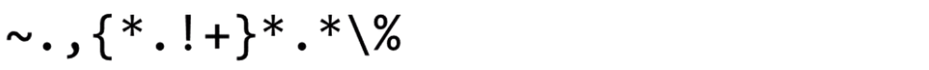
\includegraphics[width=11cm]{figures/primes_golfscript.png}}
    \end{tcolorbox}

\end{frame}
